\chapter{Analýza a rešerše}\label{analyza}

\section{Architektura apliakce}\label{analyza-architektura}

Jako doporučenou architekturu aplikací pro platformu iOS (konkrétně iPhone a iPad) uvádí Apple Model-View-Controller (zkráceně MVC).
Přestože je MVC pro vývoj aplikací nejpopulárnější, rozhodl jsem před začátkem implementace prozkoumat i jiné existující architektury.
Z alternativních architektur jsem nakonec zvolil Model-View-ViweModel, kterou porovnám s dopručeným MVC.
V závislosti na výsledku porovnání zvolím ideální architekturu pro svou aplikaci.

\subsection{MVC: Model-View-Controller}\label{analyza-mvc}
Tato architektura rozděluje aplikaci do tří vrstev: Model, View a Controller.

\subsubsection{Popis architektury}

\begin{description}
  \item[Model] reprezentuje perzistentní objekty, které aplikace využívá pro vnitřní logiku a prezentaci dat uživateli.
  Každý modelový objekt může být v relaci s libovolným počtem jiných modelových objektů.
  Tato vrstva je často reprezentována databází, příkladem mohou být databáze CoreData, Realm nebo SQLite.

  \item[View] je datový objekt viditelný uživatelem. View obsahuje logiku pro vykreslení a interakci s uživatelem.
  Přestože se View standardně používá pro zobrazení modelových objektů nebo jejich úpravu, jsou od sebe tyto vrstvy striktně odstíněny.
  Na platformě iOS tuto vrstvu reprezentuje framework UIKit vytvořený Applem.

  \item[Controller] je aplikační vrstva, která na základě vstupů z View aktualizuje a mění Model nebo překresluje View v případě, že zobrazovaná data už nejsou aktuální.
  Jedním z úkolů Controlleru je striktně zamezit přímé interakci mezi View a Modelem.
  Toto oddělení je zavedeno proto, aby View nemuselo znát konkrétní strukturu Modelu a aby Model nemusel obsahovat logiku formátování dat (cena, čas, ...) pro vykreslení.
  Dále se stará o navigaci mezi obrazovkami, síťování a interakci s uživatelem.
  Při rozdělení do obrazovek platí pravidlo, že jeden controller obsluhuje jedno nebo více View.
  Ke korektnímu vykreslení View využívá libovoné množství modelových objektů.
  O jednu obrazovku se typicky stará právě jeden Controller, je ale možné jich použít více.
\end{description}

\begin{figure}\centering
	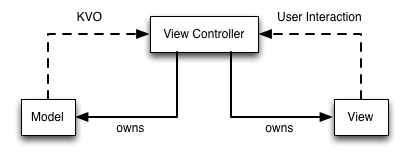
\includegraphics[width=0.5\textwidth]{assets/mvc-architecture.png}
	\caption[Architektura MVC]{Architektura MVC}\label{fig:architektura-mvc}
\end{figure}

Z tohoto shrnutí vyplývá, že Controller je velmi blízce spjat s View. Toto propojení reprezentuje obrázek \ref{fig:massive-mvc}.

\begin{figure}\centering
	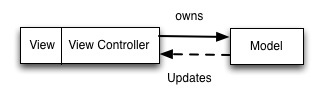
\includegraphics[width=0.5\textwidth]{assets/mvc-massive-view-controller.png}
	\caption[Role Controlleru v MVC]{Controller spjatý s View}\label{fig:massive-mvc}
\end{figure}

\subsubsection{Modelový příklad použití}

Pro možné porovnání architektury jsem připravil scénář stažení libovolných dat na základě požadavku uživatele.
V MVC by se architektura chovala takto:

\begin{itemize}
  \item Uživatel v aplikaci klikne na tlačítko \uv{Stáhnout data}.
  \item Tuto interakci odchytí view a upozorní controller.
  \item Controller na základě upozornění stáhne data a předá je modelu k uložení.
  \item Model ukládá data a notifikuje controller o změně.
  \item Controller aktualizuje view.
  \item Nastane-li během stahování chyba, controller vytváří nové view a chybu prezentuje uživateli.
\end{itemize}

\subsubsection{Shrnutí}

Shrneme-li vlastnosti vrstev, jejich klíčové role jsou:

\begin{itemize}
  \item Model udává, jakým způsobem jsou data uložena,
  \item View se stará o správné vykreslení předformátovaných dat,
  \item Controller se stará o ostatní logiku.
\end{itemize}

Pro zmíněné notifikace nabízí Apple řešení pomocí Delegate pattern.
Controller musí naimplementovat specifické rozhraní, čímž se stane delegátem.
Jako delegát se pak může zaregistrovat na notifikace obejktů, jejichž rozhraní implementoval.

MVC je v době psaní této práce nejpoužívanější architekturou a to především díky své jednoduchosti.
Při tvorbě větších aplikací ale nemusí být vhodné.
Controller se při nestandradním grafickém návrhu může stát velmi složitým, což výrazně snižuje jeho čitelnost a testovatelnost.
Z tohoto důvodu se MVC často přezdívá \uv{Massive View Controller}.
Díky přímému napojení controlleru na View se při testování chování Controlleru (behavioral testing) musí využít simulátoru mobilního operačního systému a aplikaci v něm automaticky \uv{proklikat}.
To zvyšuje časovou náročnost testování, dokonce v některých případech znemožňuje testování úplně (controlleru nezle podvrhnout mock objekty).
Tento problém se snaží řešit architektura MVVM od společnosti Microsoft.

\subsection{MVVM: Model-View-ViewModel}\label{analyza-mvvm}

Z důvodu nárustu nároků na mobilní aplikace se v posledních letech rozmáhá architektura MVVM.
Tato architektura vychází ze zmíněného MVC a jejím základním úkolem je zjednodušit Controller.

\subsubsection{Popis architektury}

Za účelem zjednodušení Controlleru se ke stávajícím třem vrstvám přidává View Model, který se stará o přípravu dat z Modelu pro zobrazení a také o perzistenci změn.

\begin{description}
  \item[View Model] je objekt vlastněný controllerem za pomoci kompozice.
  Pro Controller připravuje naformátované výstupy a poskytuje mu rozhraní pro vstupy.
  Výstupem se rozumí veškerá data, která jsou potřebná pro sestavení View.
  To může být např. datum ve specifickém formátu, cena včetně měny nebo informace o tom, kolik řádků bude obsahovat tabulka na obrazovce.
  Oproti MVC tedy perzistentní data nejsou viditelná Controlleru, ale pouze View Modelu.
  Ten je nejdříve připraví pro zobrazení.
  Vstupem může být libovolná interakce uživatele:
  změna textu v textovém poli, stisknutí tlačítka, ale i fyzický pohyb telefonem (otočení obrazovky).
  Na základě vstupů spouští View Model svou vnitřní logiku a generuje výstupy.
\end{description}

Zodpovědnost Controlleru se zavedením View Modelu dramaticky snižuje.
V ideálním případě je Controller zodpovědný pouze za správné sestavení View a napojení zfromátovaných výstupů na něj.
Dále pak za odchycení uživatelských interakcí a jejich propagaci do View Modelu.
Toto chování zachycuje obrázek \ref{architektura-mvvm}.

\begin{figure}\centering
	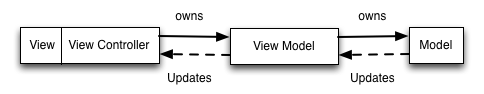
\includegraphics[width=0.5\textwidth]{assets/mvvm-architecture.png}
	\caption[Architektura MVVM]{Architektura MVVM}\label{architektura-mvvm}
\end{figure}

\subsubsection{Modelový příklad použití}

Pro porovnání architektury s MVC lze opět využít scénář pro stažení dat. Pro tento scénář by se architektura MVVM chovala následovně:
\begin{itemize}
  \item Controller napojuje výstupy view modelu na view a vytváří pravidla pro převod uživatelské interakce na vstupy view modelu.
  \item Uživatel v aplikaci klikne na tlačítko "Stáhnout data".
  \item View upozorňuje controller na interakci uživatele, ten automaticky vytváří vstup pro view model.
  \item View model na základě vstupu stahuje data a předává je modelu.
  \item Model po uložení notifikuje view model, ten vytváří výstup pro controller, který nechává překreslit view.
  \item V případě chyby vytvoří view model chybový výstup, ten se pomocí controlleru propaguje do view.
\end{itemize}

\subsubsection{Shrnutí}

Vrstvy mají následující klíčové vlastnosti:
\begin{itemize}
  \item Model definuje jakým způsobem jsou data uložena a při změně notifikuje View Model,
  \item View vykresluje na obrazovku naformátované výstupy a upozorňuje controller při interakci uživatele,
  \item Controller sestavuje hierarchii view, napojuje zformátované výstupy view modelu na view a z uživatelské interakce vytváří vstupy pro view model,
  \item View model načítá data modelu, na základě vstupů z controlleru nebo změny modelu generuje výstupy pro controller.
\end{itemize}

Oproti MVC je na tomto příkladu vidět snížení zodpovědnosti controlleru. Tato zodpovědnost se přesunula do View Modelu.
Na první pohled nemusí být tato změna opodstatněná, protože logika aplikace nezmizela, jen se přesunula.
Právě to ale umožnilo (nebo minimálně zjednodušilo) způsob, jakým lze logiku testovat.
View Model generuje výstupy na základě vstupů, v testech tedy lze uživatelskou interakci podvrhnout a testovat pouze výstupy (není potřeba vytvářet View ani Controller).
Dodatečně lze otestovat i uživatelské rozhraní.
Protože logika aplikace je otestována pomocí testů View Modelu, uživatelské rozhraní už stačí otestovat např. shodou View s referenčním obrázkem.

Při pohledu na notifikace je vidět, že přibyl typ, který nebyl v MVC potřeba.
Jedná se o notifikace směrem z View Modelu ke Controlleru (View Model nemá referenci na Controller, nemůže ho notifikovat přímo).
Některé výstupy view modelu je tedy potřeba sledovat v čase a na jejich změny reagovat.
Toto lze vyřešit pomocí KVO, které nabízí Apple v základu.
KVO umožňuje objektu zaregistrovat se na notifikace o změně stavu nějakého libovolného objektu.
V případě Controlleru by se registroval na změny stavu výstupů View Modelu.
Kdykoliv by se výstup změnil, Controller by dostal notifikaci.
Tento přístup ale není běžný pro použití s jazykem Swift.
Tento postup navíc neřeší synchronizaci vláken, z tohoto důvodu by mohlo docházet k nekonzistenci dat či neočekávanému chování.
Místo KVO se nyní standardně používají reaktivní rozšíření, které popisuji v následujících kapitolách.

Přestože mnou implementovaná aplikace není v ohledu na uživatelské scénáře nijak složitá, obsahuje mnoho obrazovek.
Obrazovky jsou vysoce interaktivní a více se k jejich implementaci hodí reaktivní přístup.
Z tohoto důvodu jsem jako architekturu vybral MVVM s použitím reaktivních rozšíření místo standardního MVC.
